\section{Simulerings blokker}
\thispagestyle{fancy}


For å skape eit meir realistisk miljø for testinga lagde vi nokre simuleringsblokker.
Desse blokkene etterlignar driftssituasjonar og gjer simuleringa enklare og betre.
Vi lagde i hovudsak to slike blokker, ei blokk som simulerer fylling av ein tank
og ei blokk som simulerer tilbakemelding frå ventilar.

Blokk for tank simulering er enkel og skreven spesfikt for Sande reiseanlegg med ein mottakstank
og to reaktorar.
Det er usansyneleg at desse simuleringsblokkene vil bli brukt vidare, men dei gav
oss den realismen vi trengte.

Blokkene er også med å gjere sjølve arbeidet med simuleringa enklare.
Før vi lage blokk for tilbakemelding på ventilar, 
gav vi manuelt kvar ventil XGH eller XHL basert på kor den eigentleg skulle være (open/lukka).
Dette fungerer greit dersom ein tester små områder eller kun ein ventilblokk, men
når ein simulerer ein større grad av programmet blir denne jobben tidkrevjande.

På desse blokkene har vi tatt oss meir friheit i namngiving, feilhandtering osv
fordi blokkene ikkje skal brukast når programmet er ferdig.

\begin{figure}[htbp]
    \centering
    \begin{subfigure}[b]{0.3\textwidth}
        \centering
        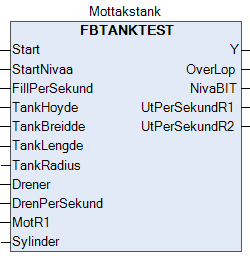
\includegraphics[width=0.9\textwidth]{Figurar/TankSim.png}
        \caption{Tank}\label{fig:TankSim}
    \end{subfigure}
    \hfill
    \begin{subfigure}[b]{0.3\textwidth}
        \centering
        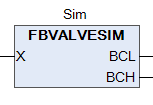
\includegraphics[width=0.9\textwidth]{Figurar/ValveSim.png}
        \caption{Ventil}\label{fig:ValveSim}
    \end{subfigure}
    \caption{Simuleringsblokker}\label{fig:SimuleringsBlokker}
\end{figure}

\newpage